%\documentclass[12pt,handout]{beamer}
\documentclass{beamer}
\usepackage[ngerman]{babel}
\usepackage[utf8]{inputenc}
\usepackage{amsmath}
\usepackage{amssymb}
\usepackage{listings} 
\usepackage{mathtools}
\usepackage{ulem}
\usetheme{Boadilla}

\parskip 10pt

\begin{document}
\title{Komplexität}   
\author{Informatik} 
\date{ } 
\lstset{language=Python, tabsize=4, showstringspaces=false,basicstyle=\footnotesize,mathescape=true}
\lstset{literate=%
  {Ö}{{\"O}}1
  {Ä}{{\"A}}1
  {Ü}{{\"U}}1
  {ß}{{\ss}}1
  {ü}{{\"u}}1
  {ä}{{\"a}}1
  {ö}{{\"o}}1
}

\frame{\titlepage} 

%---

\begin{frame}[fragile]
Die \textbf{Komplexität} eines Algorithmus bezieht sich auf die Frage, wieviel Zeit er für seine Arbeit benötigt. \pause

Nicht: absolute CPU-Zeit angeben \\
Nicht: Anzahl der Maschinenbefehle zählen  

Sondern:  Wachstum der Laufzeit in Abhängigkeit
 von der Größe der Eingabe

Größe der Eingabe kann z.B. sein: Zahl der Daten,  Wert der Eingabezahl,   Länge der Codierung. 
\end{frame}

%---
\begin{frame}[fragile]
Uns interessiert die Größenordnung dieser Änderung.  Dazu nutzen wir die O-Notation.  

$f(n) \in O(n^2) \Rightarrow$  wenn sich die Eingabegröße verdoppelt, \pause vervierfacht sich (ungefähr) die Laufzeit.  
Wenn sich die Eingabegröße verdreifacht, \pause verneunfacht sich die Laufzeit. 

$f(n) \in O(n) \Rightarrow$  wenn sich die Eingabegröße verdoppelt, \pause verdoppelt sich die Laufzeit. 

$f(n) \in O(2^n) \Rightarrow$  wenn sich die Eingabegröße um 10 erhöht, \pause vertausendfacht ($\approx 1024$) sich die Laufzeit. 

$f(n) \in O($log n$) \Rightarrow$  wenn sich die Eingabegröße verdoppelt, \pause erhöht sich die Laufzeit um 1. 

$f(n) \in O(1)  \Rightarrow$  \pause die Laufzeit ist unabhängig von der Größe der Eingabe.
\end{frame}

%---

\begin{frame}[fragile]
Im O-Kalkül interessiert nur die Funktion, die bei großem n das Wachstum dominiert. Faktoren und weniger schnell wachsende Terme werden vernachlässigt.  

$f(n) = 3n^2 + 4n + 7  \in \pause O(n^2)$  \\ 
$f(n) = 1000n^2 \in \pause O(n^2)$  \\  
$f(n) =20n + 4 \cdot 2^n \in \pause O(2^n)$ \\  
$f(n) =n + 2 \cdot \log n \in \pause O(n)$ \\ 

\end{frame}

\section{Logarithmus}
%---
\begin{frame}[fragile]
In der Informatik nutzen wir standardmäßig den Logarithmus zur Basis 2. 
$\log x = \log_{2} x = $ die Zahl, hoch die ich 2 nehmen muss, um zu x zu gelangen. \pause

$\log 1 =  0$ denn $2^0 = 1$  \\ 
$\log 2 = 1$ denn $2^1 = 2$ \\ 
$\log 4 = 2$ denn $2^2 = 4$  \\ 
$\log 8 =  3$ denn $2^3 = 8$  

Wenn sich das Argument verdoppelt, \pause erhöht sich der Logarithmus um 1 \\ 
Wenn sich das Argument halbiert, \pause erniedrigt sich der Logarithmus um 1. 

Der ganzzahlige Logarithmus gibt an, wie oft ich eine Zahl halbieren muss, um zu einer 1 vor dem Komma zu gelangen.

Wenn ein Algorithmus in der Komplexitätsklasse $O(\log n)$ ist und die Eingabegröße wird vertausendfacht,  dann wächst die Laufzeit um \pause 10 Schritte. \pause Wächst die Eingabegröße um das millionenfache,  dann wächst die Laufzeit um \pause 20 Schritte.

\end{frame}

%--

\begin{frame}[fragile]

Annahme: 1 Schritt dauert $1 \mu s = 0.000001 s$

\begin{tabular}{l | l l l l l l}
$n =   $   &   10 & 20 & 30 & 40 & 50 & 60 \\
\hline
$\log n$ & $3.3\mu s$  & $4.3\mu s$ & $4.9\mu s$  & $5.3\mu s$ & $5.6\mu s$ &  $5.9\mu s$ \\ \pause
$n$ & $10\mu s$  & $20\mu s$ & $30\mu s$  & $40\mu s$ & $50\mu s$ &  $60\mu s$ \\ \pause
$n \cdot \log n $ & $33\mu s$  & $86\mu s$ & $147\mu s$  & $212\mu s$ & $280\mu s$ &  $354\mu s$ \\ \pause
$n^2  $ & $100\mu s$  & $400\mu s$ & $900\mu s$  & $1.6ms $ & $2.5ms$ &  $3.6 ms$ \\ \pause
$n^3  $ & $1ms$  & $8ms$ & $27ms$  & $64ms $ & $125ms$ &  $216 ms$ \pause \\ 
\hline
$2^n  $ & $1ms$  & $1s$ & $18min$  & $13\text{ Tage}$ & $36 J$ &  $366Jh$ \\ \pause
$3^n  $ & $59ms$  & $58min$ & $6,5J$  & $3855Jh$ & $10^8 Jh$ &  $10^{13} Jh$ \\ \pause
$n!  $ & $6.62s $  & $771 Jh$ & $10^{16} Jh$  &  $10^{32} Jh$ &  $10^{49} Jh$ &  $10^{66} Jh$ \\
\hline
\end{tabular} 


Alter des Universums: ca. 15 Mrd. Jahre =   $ 1,5 \cdot 10^9 J =   1,5 \cdot 10^7 Jh$  

Algorithmen, die exponentielle oder stärkere Laufzeiten haben, sind in der Regel nicht praktikabel (nicht effizient).

\end{frame}

\begin{frame}[fragile]
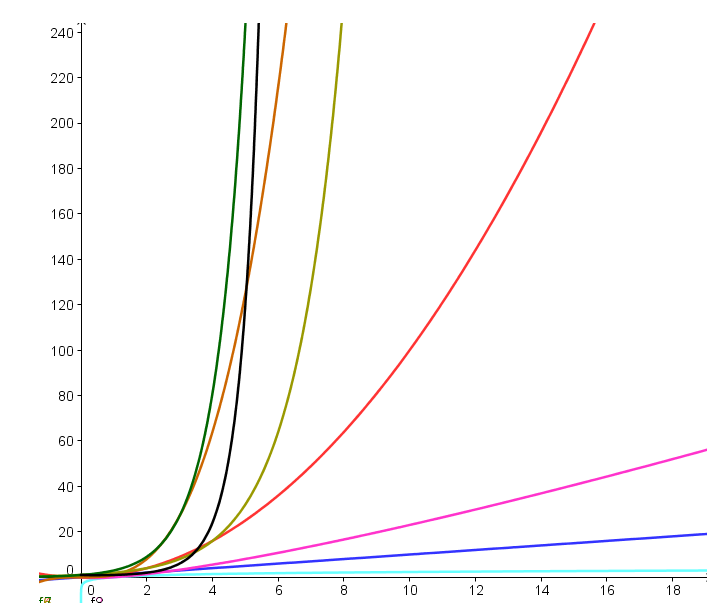
\includegraphics[height=8cm]{kurven.png}
Wachstumskurven für $x, x^2, x^3, \log(x), x\log(x), 2^x, 3^x, x!$
\end{frame}
\begin{frame}[fragile]
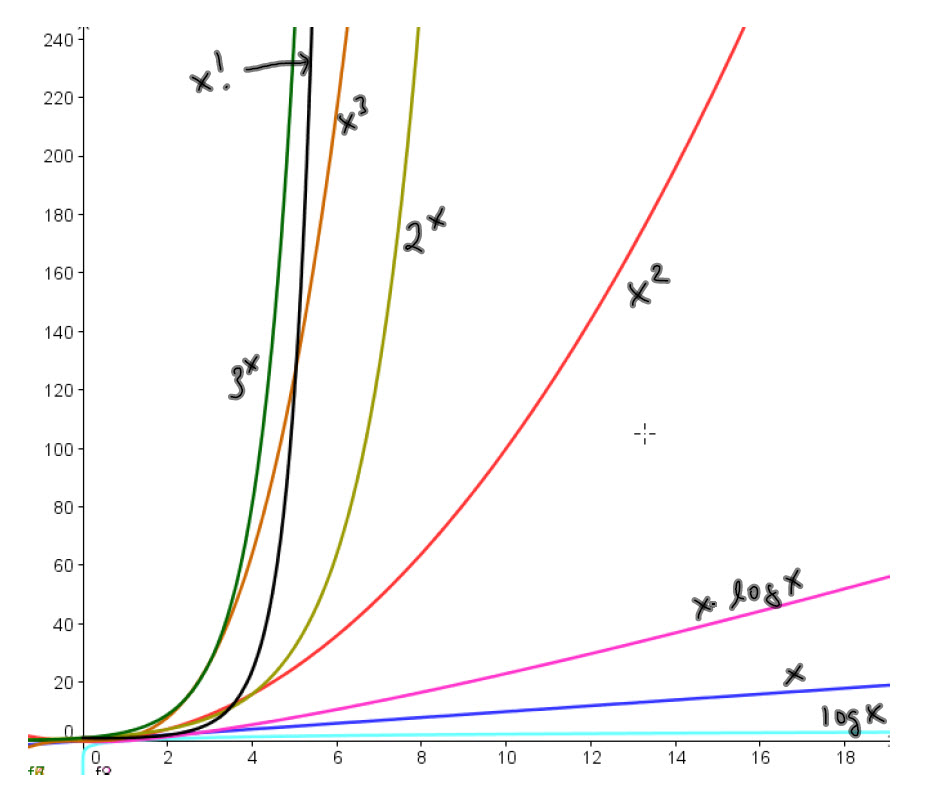
\includegraphics[height=8cm]{bild2.jpg}
Wachstumskurven für $x, x^2, x^3, \log(x), x\log(x), 2^x, 3^x, x!$
\end{frame}
%--
\section{Komplexitätsklassen}
\begin{frame}[fragile]

Beispiele für Komplexitätsklassen  

\begin{tabular}{ll}
$O(\log n)$   &  binäre Suche  \\ 
$O(n)$   &  lineare Suche  \\ 
$O(n \cdot \log n)$   &  schlaues Sortieren  \\  
$O(n^2)$   &  dummes Sortieren  \\  
$O(2^n)$   &  alle Teilmengen \\ 
$O(n!)$   &  alle Permutationen  
\end{tabular}
\end{frame}

\begin{frame}[fragile]
Analoge Komplexitätsaussagen sind möglich bzgl. Speicherplatz. \\
Wir zählen nicht die Anzahl der Bytes, sondern betrachten das Wachstum des Platzbedarfs 
 in Abhängigkeit von der Größe der Eingabe.  \pause

Aussagen über Laufzeit und Platzbedarf sind möglich für den
\begin{itemize}
\item best case
\item worst case 
\item average case
\end{itemize}

\end{frame}


\section{Beispiele}
\begin{frame}[fragile]
Beispiel1 : Minimumsuche in einer Liste a der Länge n.  

\begin{lstlisting} 
def minimum(a): $\pause$
    min = a[0]
    for i in range(len(a)):
        if a[i] < min:
            min = a[i]
    return min
\end{lstlisting}  

best case: \pause $O(n)$  ~~~    worst case:    $O(n)$    ~~~ average case:   $O(n)$  
\end{frame}


\begin{frame}[fragile]
Beispiel2 :  Gibt es doppelte Elemente in einer Liste a der Länge n? 
\begin{lstlisting} 
def doppelte(a): $\pause$
    n = len(a)   
    for i in range(n-1):
        for j in range(i+1,n):
            if a[i] $==$ a[j]:
                return True
    return False

\end{lstlisting}  

best case: \pause $O(1)$  ~~~   worst case:   $O(n^2)$
\end{frame}
 \end{document}